% Systematisk beskrivelse af konfigurations tabel.
\section{Konfigurationstabel}\label{konfigurationstabel}
En konfiguration af et system er en kombination af beslutninger relateret til systemets opbygning, dette inkluderer beslutninger om målgruppe, systemkoncept, komponenter og mere.
En konfigurationstabel er så en tabel med en sådan konfiguration, hvor konfigurationen er inddelt i de fire kategorier Paradigm, Product, Project og Process \citep{art:essence}.
I \cref{tab:konfigurationsTabel} præsenteres konfigurationstabellen for projektet, og indholdet vil i de følgende afsnit blive forklaret.

\begin{figure}
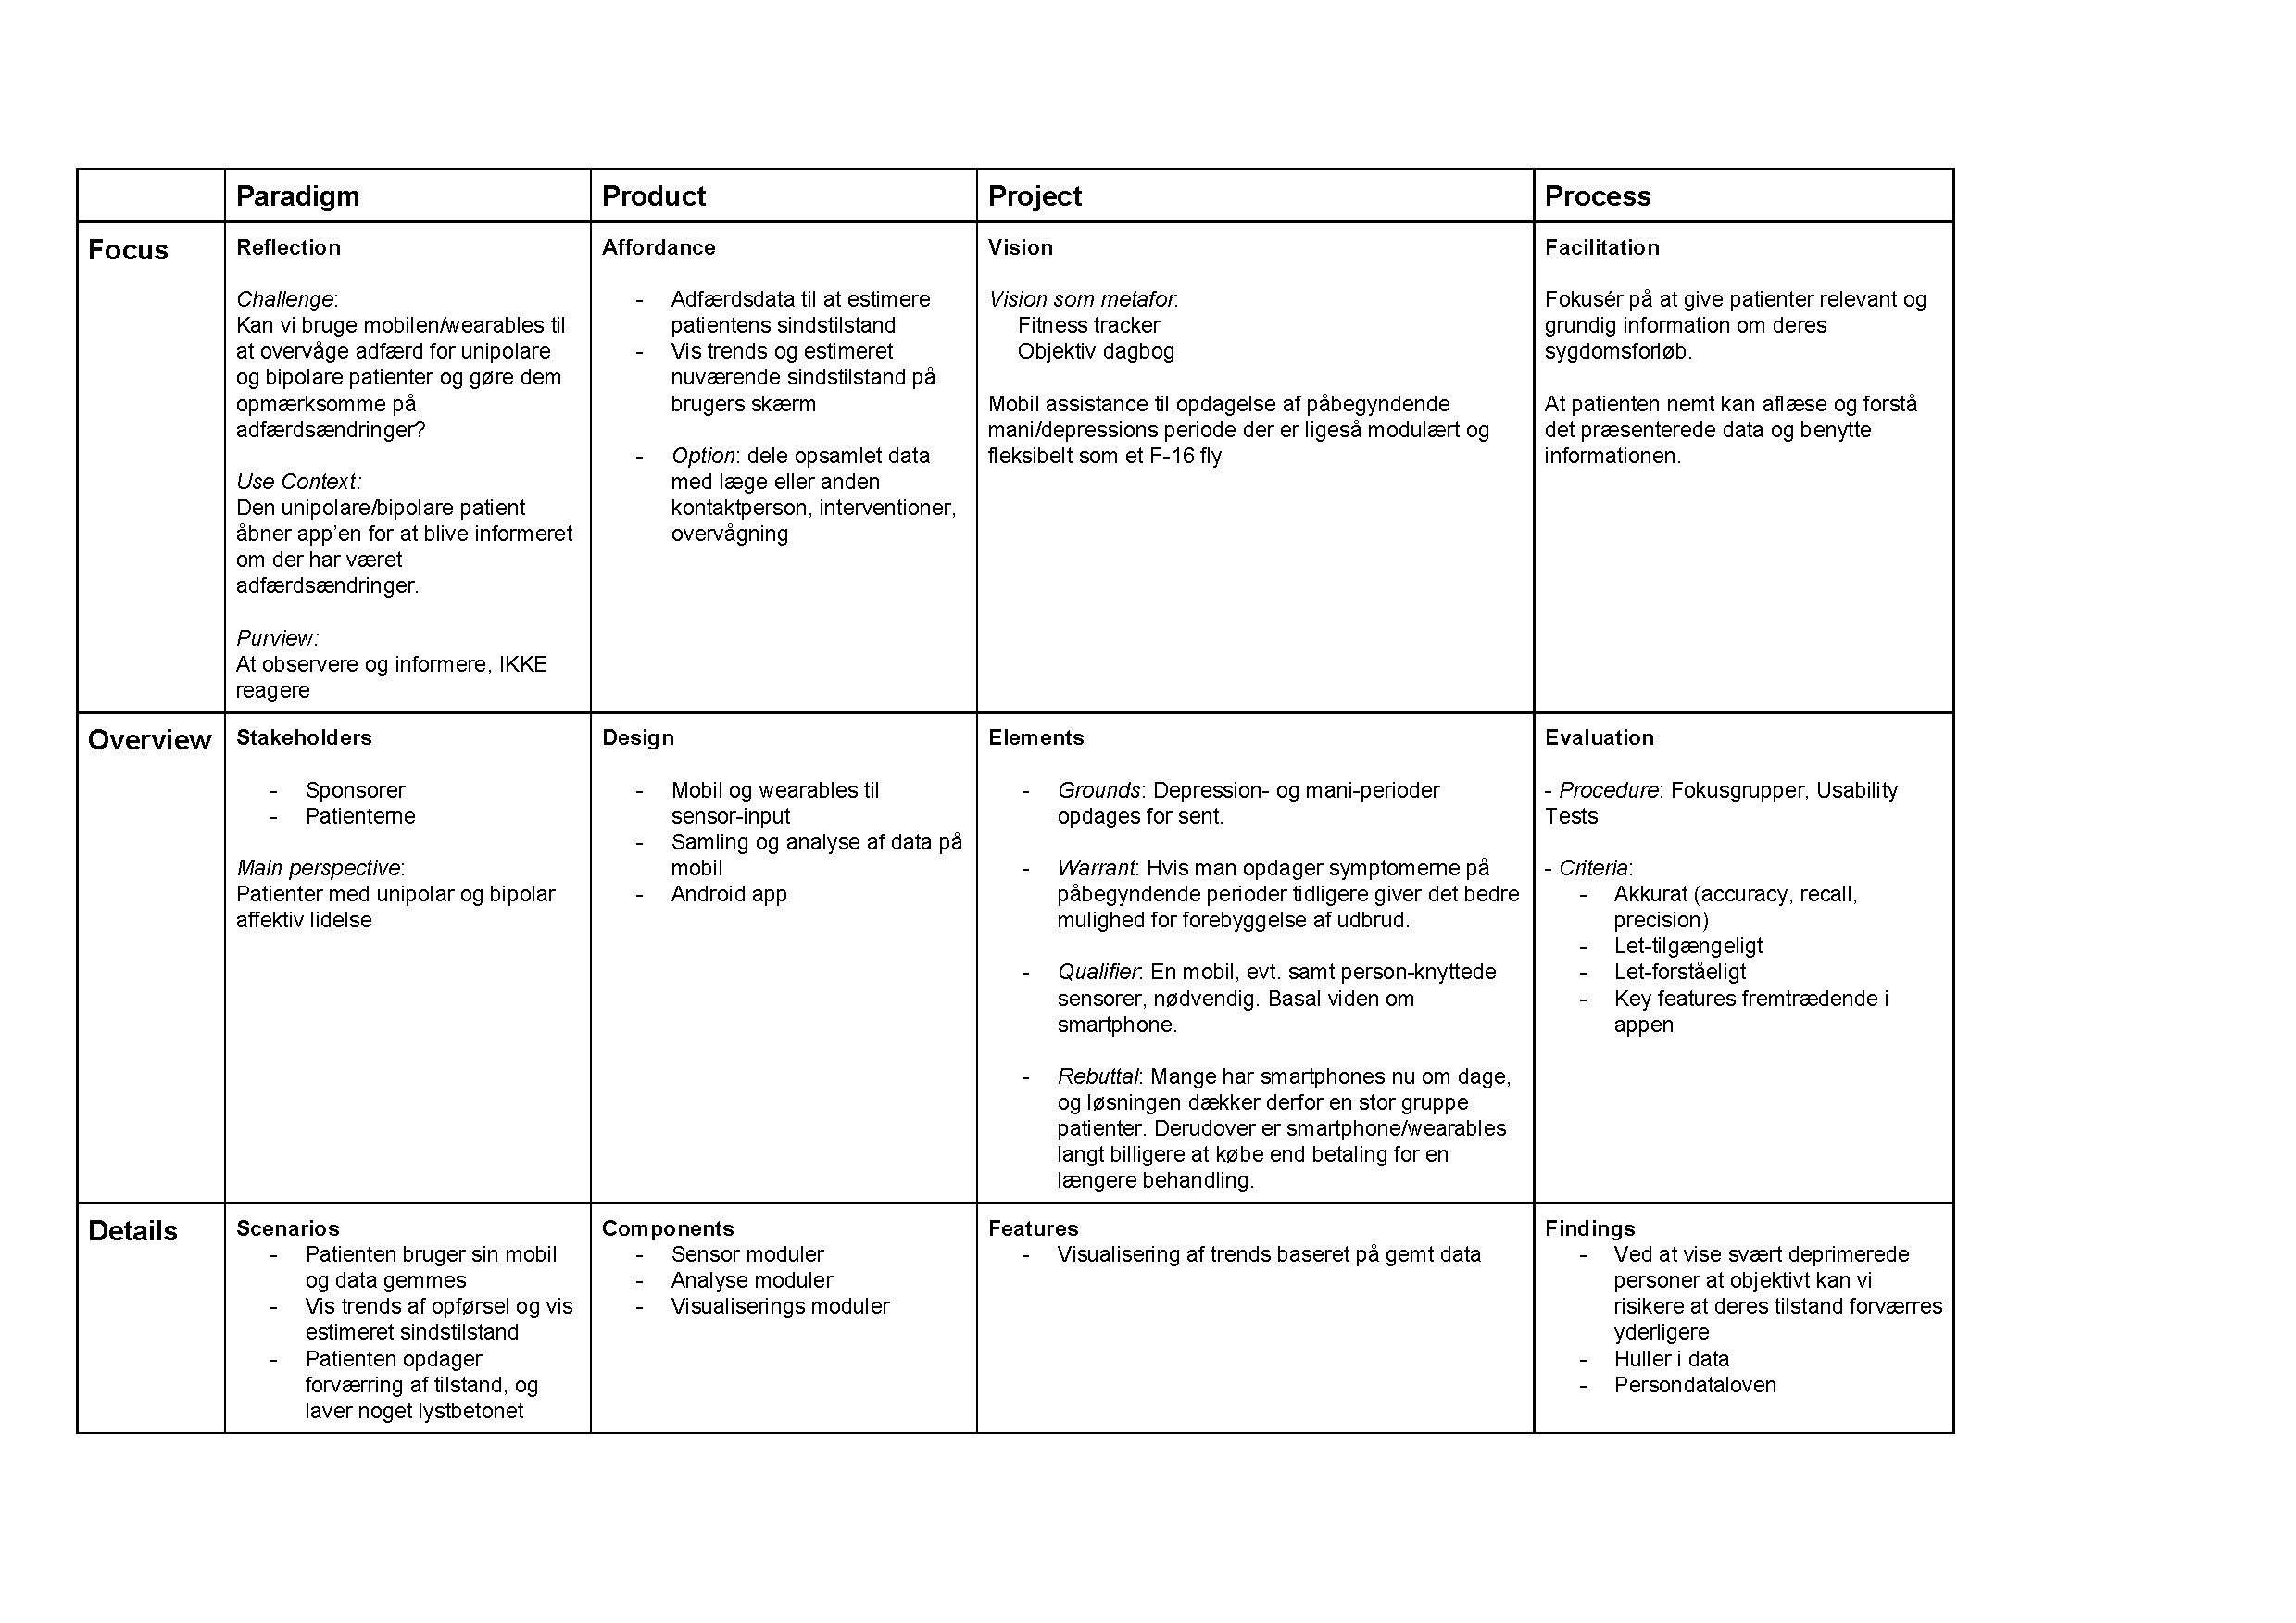
\includegraphics[scale = 0.65,trim = 1cm 3cm 6cm 2cm, angle = 90, clip]{KonfigurationTabel}
\caption{Konfigurations tabellen for systemet.}
\label{tab:konfigurationsTabel}
\end{figure}
